% Created by tikzDevice version 0.10.1 on 2017-12-07 15:49:08
% !TEX encoding = UTF-8 Unicode
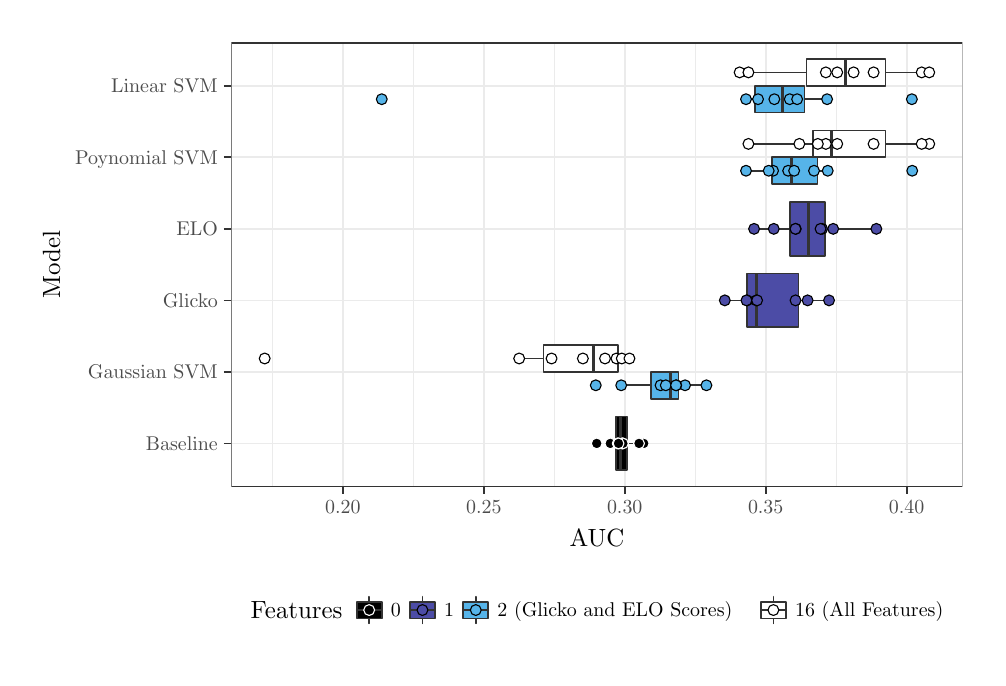
\begin{tikzpicture}[x=1pt,y=1pt]
\definecolor{fillColor}{RGB}{255,255,255}
\path[use as bounding box,fill=fillColor,fill opacity=0.00] (0,0) rectangle (343.28,227.65);
\begin{scope}
\path[clip] (  0.00,  0.00) rectangle (343.28,227.65);
\definecolor{drawColor}{RGB}{255,255,255}
\definecolor{fillColor}{RGB}{255,255,255}

\path[draw=drawColor,line width= 0.6pt,line join=round,line cap=round,fill=fillColor] (  0.00,  0.00) rectangle (343.28,227.65);
\end{scope}
\begin{scope}
\path[clip] ( 73.64, 61.91) rectangle (337.78,222.15);
\definecolor{fillColor}{RGB}{255,255,255}

\path[fill=fillColor] ( 73.64, 61.91) rectangle (337.78,222.15);
\definecolor{drawColor}{gray}{0.92}

\path[draw=drawColor,line width= 0.3pt,line join=round] ( 88.40, 61.91) --
	( 88.40,222.15);

\path[draw=drawColor,line width= 0.3pt,line join=round] (139.34, 61.91) --
	(139.34,222.15);

\path[draw=drawColor,line width= 0.3pt,line join=round] (190.28, 61.91) --
	(190.28,222.15);

\path[draw=drawColor,line width= 0.3pt,line join=round] (241.22, 61.91) --
	(241.22,222.15);

\path[draw=drawColor,line width= 0.3pt,line join=round] (292.16, 61.91) --
	(292.16,222.15);

\path[draw=drawColor,line width= 0.6pt,line join=round] ( 73.64, 77.42) --
	(337.78, 77.42);

\path[draw=drawColor,line width= 0.6pt,line join=round] ( 73.64,103.27) --
	(337.78,103.27);

\path[draw=drawColor,line width= 0.6pt,line join=round] ( 73.64,129.11) --
	(337.78,129.11);

\path[draw=drawColor,line width= 0.6pt,line join=round] ( 73.64,154.95) --
	(337.78,154.95);

\path[draw=drawColor,line width= 0.6pt,line join=round] ( 73.64,180.80) --
	(337.78,180.80);

\path[draw=drawColor,line width= 0.6pt,line join=round] ( 73.64,206.64) --
	(337.78,206.64);

\path[draw=drawColor,line width= 0.6pt,line join=round] (113.87, 61.91) --
	(113.87,222.15);

\path[draw=drawColor,line width= 0.6pt,line join=round] (164.81, 61.91) --
	(164.81,222.15);

\path[draw=drawColor,line width= 0.6pt,line join=round] (215.75, 61.91) --
	(215.75,222.15);

\path[draw=drawColor,line width= 0.6pt,line join=round] (266.69, 61.91) --
	(266.69,222.15);

\path[draw=drawColor,line width= 0.6pt,line join=round] (317.63, 61.91) --
	(317.63,222.15);
\definecolor{drawColor}{gray}{0.20}

\path[draw=drawColor,line width= 0.6pt,line join=round] (216.54, 77.42) -- (220.91, 77.42);

\path[draw=drawColor,line width= 0.6pt,line join=round] (212.54, 77.42) -- (210.53, 77.42);
\definecolor{fillColor}{RGB}{0,0,0}

\path[draw=drawColor,line width= 0.6pt,line join=round,line cap=round,fill=fillColor] (216.54, 67.73) --
	(212.54, 67.73) --
	(212.54, 87.11) --
	(216.54, 87.11) --
	(216.54, 67.73) --
	cycle;

\path[draw=drawColor,line width= 1.1pt,line join=round] (214.17, 67.73) -- (214.17, 87.11);

\path[draw=drawColor,line width= 0.6pt,line join=round] (235.17, 98.42) -- (245.27, 98.42);

\path[draw=drawColor,line width= 0.6pt,line join=round] (225.14, 98.42) -- (214.47, 98.42);
\definecolor{fillColor}{RGB}{86,180,233}

\path[draw=drawColor,line width= 0.6pt,line join=round,line cap=round,fill=fillColor] (235.17, 93.57) --
	(225.14, 93.57) --
	(225.14,103.27) --
	(235.17,103.27) --
	(235.17, 93.57) --
	cycle;

\path[draw=drawColor,line width= 1.1pt,line join=round] (232.42, 93.57) -- (232.42,103.27);

\path[draw=drawColor,line width= 0.6pt,line join=round] (213.24,108.11) -- (217.45,108.11);

\path[draw=drawColor,line width= 0.6pt,line join=round] (186.37,108.11) -- (177.60,108.11);
\definecolor{fillColor}{RGB}{255,255,255}

\path[draw=drawColor,line width= 0.6pt,line join=round,line cap=round,fill=fillColor] (213.24,103.27) --
	(186.37,103.27) --
	(186.37,112.96) --
	(213.24,112.96) --
	(213.24,103.27) --
	cycle;

\path[draw=drawColor,line width= 1.1pt,line join=round] (204.62,103.27) -- (204.62,112.96);

\path[draw=drawColor,line width= 0.6pt,line join=round] (278.55,129.11) -- (289.57,129.11);

\path[draw=drawColor,line width= 0.6pt,line join=round] (259.92,129.11) -- (251.91,129.11);
\definecolor{fillColor}{RGB}{76,76,166}

\path[draw=drawColor,line width= 0.6pt,line join=round,line cap=round,fill=fillColor] (278.55,119.42) --
	(259.92,119.42) --
	(259.92,138.80) --
	(278.55,138.80) --
	(278.55,119.42) --
	cycle;

\path[draw=drawColor,line width= 1.1pt,line join=round] (263.45,119.42) -- (263.45,138.80);

\path[draw=drawColor,line width= 0.6pt,line join=round] (288.07,154.95) -- (306.67,154.95);

\path[draw=drawColor,line width= 0.6pt,line join=round] (275.47,154.95) -- (262.48,154.95);

\path[draw=drawColor,line width= 0.6pt,line join=round,line cap=round,fill=fillColor] (288.07,145.26) --
	(275.47,145.26) --
	(275.47,164.65) --
	(288.07,164.65) --
	(288.07,145.26) --
	cycle;

\path[draw=drawColor,line width= 1.1pt,line join=round] (282.03,145.26) -- (282.03,164.65);

\path[draw=drawColor,line width= 0.6pt,line join=round] (285.39,175.95) -- (289.10,175.95);

\path[draw=drawColor,line width= 0.6pt,line join=round] (268.95,175.95) -- (259.57,175.95);
\definecolor{fillColor}{RGB}{86,180,233}

\path[draw=drawColor,line width= 0.6pt,line join=round,line cap=round,fill=fillColor] (285.39,171.11) --
	(268.95,171.11) --
	(268.95,180.80) --
	(285.39,180.80) --
	(285.39,171.11) --
	cycle;

\path[draw=drawColor,line width= 1.1pt,line join=round] (275.88,171.11) -- (275.88,180.80);

\path[draw=drawColor,line width= 0.6pt,line join=round] (310.01,185.65) -- (325.78,185.65);

\path[draw=drawColor,line width= 0.6pt,line join=round] (283.85,185.65) -- (260.44,185.65);
\definecolor{fillColor}{RGB}{255,255,255}

\path[draw=drawColor,line width= 0.6pt,line join=round,line cap=round,fill=fillColor] (310.01,180.80) --
	(283.85,180.80) --
	(283.85,190.49) --
	(310.01,190.49) --
	(310.01,180.80) --
	cycle;

\path[draw=drawColor,line width= 1.1pt,line join=round] (290.47,180.80) -- (290.47,190.49);

\path[draw=drawColor,line width= 0.6pt,line join=round] (280.75,201.80) -- (288.87,201.80);

\path[draw=drawColor,line width= 0.6pt,line join=round] (262.83,201.80) -- (259.57,201.80);
\definecolor{fillColor}{RGB}{86,180,233}

\path[draw=drawColor,line width= 0.6pt,line join=round,line cap=round,fill=fillColor] (280.75,196.95) --
	(262.83,196.95) --
	(262.83,206.64) --
	(280.75,206.64) --
	(280.75,196.95) --
	cycle;

\path[draw=drawColor,line width= 1.1pt,line join=round] (272.59,196.95) -- (272.59,206.64);

\path[draw=drawColor,line width= 0.6pt,line join=round] (310.01,211.49) -- (325.78,211.49);

\path[draw=drawColor,line width= 0.6pt,line join=round] (281.43,211.49) -- (257.26,211.49);
\definecolor{fillColor}{RGB}{255,255,255}

\path[draw=drawColor,line width= 0.6pt,line join=round,line cap=round,fill=fillColor] (310.01,206.64) --
	(281.43,206.64) --
	(281.43,216.34) --
	(310.01,216.34) --
	(310.01,206.64) --
	cycle;

\path[draw=drawColor,line width= 1.1pt,line join=round] (295.49,206.64) -- (295.49,216.34);
\definecolor{drawColor}{RGB}{255,255,255}
\definecolor{fillColor}{RGB}{0,0,0}

\path[draw=drawColor,line width= 0.4pt,line join=round,line cap=round,fill=fillColor] (205.62, 77.42) circle (  1.96);

\path[draw=drawColor,line width= 0.4pt,line join=round,line cap=round,fill=fillColor] (214.84, 77.42) circle (  1.96);

\path[draw=drawColor,line width= 0.4pt,line join=round,line cap=round,fill=fillColor] (210.53, 77.42) circle (  1.96);

\path[draw=drawColor,line width= 0.4pt,line join=round,line cap=round,fill=fillColor] (215.08, 77.42) circle (  1.96);

\path[draw=drawColor,line width= 0.4pt,line join=round,line cap=round,fill=fillColor] (213.21, 77.42) circle (  1.96);

\path[draw=drawColor,line width= 0.4pt,line join=round,line cap=round,fill=fillColor] (222.61, 77.42) circle (  1.96);

\path[draw=drawColor,line width= 0.4pt,line join=round,line cap=round,fill=fillColor] (220.91, 77.42) circle (  1.96);

\path[draw=drawColor,line width= 0.4pt,line join=round,line cap=round,fill=fillColor] (213.51, 77.42) circle (  1.96);
\definecolor{drawColor}{RGB}{0,0,0}
\definecolor{fillColor}{RGB}{255,255,255}

\path[draw=drawColor,line width= 0.4pt,line join=round,line cap=round,fill=fillColor] (212.76,108.11) circle (  1.96);

\path[draw=drawColor,line width= 0.4pt,line join=round,line cap=round,fill=fillColor] (214.67,108.11) circle (  1.96);

\path[draw=drawColor,line width= 0.4pt,line join=round,line cap=round,fill=fillColor] (208.62,108.11) circle (  1.96);

\path[draw=drawColor,line width= 0.4pt,line join=round,line cap=round,fill=fillColor] (177.60,108.11) circle (  1.96);

\path[draw=drawColor,line width= 0.4pt,line join=round,line cap=round,fill=fillColor] (189.30,108.11) circle (  1.96);

\path[draw=drawColor,line width= 0.4pt,line join=round,line cap=round,fill=fillColor] (217.45,108.11) circle (  1.96);

\path[draw=drawColor,line width= 0.4pt,line join=round,line cap=round,fill=fillColor] (200.62,108.11) circle (  1.96);

\path[draw=drawColor,line width= 0.4pt,line join=round,line cap=round,fill=fillColor] ( 85.64,108.11) circle (  1.96);
\definecolor{fillColor}{RGB}{86,180,233}

\path[draw=drawColor,line width= 0.4pt,line join=round,line cap=round,fill=fillColor] (237.54, 98.42) circle (  1.96);

\path[draw=drawColor,line width= 0.4pt,line join=round,line cap=round,fill=fillColor] (245.27, 98.42) circle (  1.96);

\path[draw=drawColor,line width= 0.4pt,line join=round,line cap=round,fill=fillColor] (228.69, 98.42) circle (  1.96);

\path[draw=drawColor,line width= 0.4pt,line join=round,line cap=round,fill=fillColor] (230.57, 98.42) circle (  1.96);

\path[draw=drawColor,line width= 0.4pt,line join=round,line cap=round,fill=fillColor] (205.28, 98.42) circle (  1.96);

\path[draw=drawColor,line width= 0.4pt,line join=round,line cap=round,fill=fillColor] (234.38, 98.42) circle (  1.96);

\path[draw=drawColor,line width= 0.4pt,line join=round,line cap=round,fill=fillColor] (234.27, 98.42) circle (  1.96);

\path[draw=drawColor,line width= 0.4pt,line join=round,line cap=round,fill=fillColor] (214.47, 98.42) circle (  1.96);
\definecolor{fillColor}{RGB}{76,76,166}

\path[draw=drawColor,line width= 0.4pt,line join=round,line cap=round,fill=fillColor] (259.98,129.11) circle (  1.96);

\path[draw=drawColor,line width= 0.4pt,line join=round,line cap=round,fill=fillColor] (263.33,129.11) circle (  1.96);

\path[draw=drawColor,line width= 0.4pt,line join=round,line cap=round,fill=fillColor] (251.91,129.11) circle (  1.96);

\path[draw=drawColor,line width= 0.4pt,line join=round,line cap=round,fill=fillColor] (289.57,129.11) circle (  1.96);

\path[draw=drawColor,line width= 0.4pt,line join=round,line cap=round,fill=fillColor] (281.83,129.11) circle (  1.96);

\path[draw=drawColor,line width= 0.4pt,line join=round,line cap=round,fill=fillColor] (259.73,129.11) circle (  1.96);

\path[draw=drawColor,line width= 0.4pt,line join=round,line cap=round,fill=fillColor] (277.46,129.11) circle (  1.96);

\path[draw=drawColor,line width= 0.4pt,line join=round,line cap=round,fill=fillColor] (263.57,129.11) circle (  1.96);

\path[draw=drawColor,line width= 0.4pt,line join=round,line cap=round,fill=fillColor] (269.60,154.95) circle (  1.96);

\path[draw=drawColor,line width= 0.4pt,line join=round,line cap=round,fill=fillColor] (287.07,154.95) circle (  1.96);

\path[draw=drawColor,line width= 0.4pt,line join=round,line cap=round,fill=fillColor] (262.48,154.95) circle (  1.96);

\path[draw=drawColor,line width= 0.4pt,line join=round,line cap=round,fill=fillColor] (277.55,154.95) circle (  1.96);

\path[draw=drawColor,line width= 0.4pt,line join=round,line cap=round,fill=fillColor] (291.07,154.95) circle (  1.96);

\path[draw=drawColor,line width= 0.4pt,line join=round,line cap=round,fill=fillColor] (286.50,154.95) circle (  1.96);

\path[draw=drawColor,line width= 0.4pt,line join=round,line cap=round,fill=fillColor] (277.43,154.95) circle (  1.96);

\path[draw=drawColor,line width= 0.4pt,line join=round,line cap=round,fill=fillColor] (306.67,154.95) circle (  1.96);
\definecolor{fillColor}{RGB}{255,255,255}

\path[draw=drawColor,line width= 0.4pt,line join=round,line cap=round,fill=fillColor] (292.53,185.65) circle (  1.96);

\path[draw=drawColor,line width= 0.4pt,line join=round,line cap=round,fill=fillColor] (260.44,185.65) circle (  1.96);

\path[draw=drawColor,line width= 0.4pt,line join=round,line cap=round,fill=fillColor] (305.67,185.65) circle (  1.96);

\path[draw=drawColor,line width= 0.4pt,line join=round,line cap=round,fill=fillColor] (288.42,185.65) circle (  1.96);

\path[draw=drawColor,line width= 0.4pt,line join=round,line cap=round,fill=fillColor] (285.52,185.65) circle (  1.96);

\path[draw=drawColor,line width= 0.4pt,line join=round,line cap=round,fill=fillColor] (325.78,185.65) circle (  1.96);

\path[draw=drawColor,line width= 0.4pt,line join=round,line cap=round,fill=fillColor] (278.84,185.65) circle (  1.96);

\path[draw=drawColor,line width= 0.4pt,line join=round,line cap=round,fill=fillColor] (323.05,185.65) circle (  1.96);
\definecolor{fillColor}{RGB}{86,180,233}

\path[draw=drawColor,line width= 0.4pt,line join=round,line cap=round,fill=fillColor] (274.80,175.95) circle (  1.96);

\path[draw=drawColor,line width= 0.4pt,line join=round,line cap=round,fill=fillColor] (269.34,175.95) circle (  1.96);

\path[draw=drawColor,line width= 0.4pt,line join=round,line cap=round,fill=fillColor] (289.10,175.95) circle (  1.96);

\path[draw=drawColor,line width= 0.4pt,line join=round,line cap=round,fill=fillColor] (319.63,175.95) circle (  1.96);

\path[draw=drawColor,line width= 0.4pt,line join=round,line cap=round,fill=fillColor] (276.96,175.95) circle (  1.96);

\path[draw=drawColor,line width= 0.4pt,line join=round,line cap=round,fill=fillColor] (259.57,175.95) circle (  1.96);

\path[draw=drawColor,line width= 0.4pt,line join=round,line cap=round,fill=fillColor] (284.15,175.95) circle (  1.96);

\path[draw=drawColor,line width= 0.4pt,line join=round,line cap=round,fill=fillColor] (267.77,175.95) circle (  1.96);
\definecolor{fillColor}{RGB}{255,255,255}

\path[draw=drawColor,line width= 0.4pt,line join=round,line cap=round,fill=fillColor] (305.67,211.49) circle (  1.96);

\path[draw=drawColor,line width= 0.4pt,line join=round,line cap=round,fill=fillColor] (257.26,211.49) circle (  1.96);

\path[draw=drawColor,line width= 0.4pt,line join=round,line cap=round,fill=fillColor] (288.42,211.49) circle (  1.96);

\path[draw=drawColor,line width= 0.4pt,line join=round,line cap=round,fill=fillColor] (260.44,211.49) circle (  1.96);

\path[draw=drawColor,line width= 0.4pt,line join=round,line cap=round,fill=fillColor] (292.53,211.49) circle (  1.96);

\path[draw=drawColor,line width= 0.4pt,line join=round,line cap=round,fill=fillColor] (298.45,211.49) circle (  1.96);

\path[draw=drawColor,line width= 0.4pt,line join=round,line cap=round,fill=fillColor] (323.05,211.49) circle (  1.96);

\path[draw=drawColor,line width= 0.4pt,line join=round,line cap=round,fill=fillColor] (325.78,211.49) circle (  1.96);
\definecolor{fillColor}{RGB}{86,180,233}

\path[draw=drawColor,line width= 0.4pt,line join=round,line cap=round,fill=fillColor] (269.81,201.80) circle (  1.96);

\path[draw=drawColor,line width= 0.4pt,line join=round,line cap=round,fill=fillColor] (288.87,201.80) circle (  1.96);

\path[draw=drawColor,line width= 0.4pt,line join=round,line cap=round,fill=fillColor] (275.37,201.80) circle (  1.96);

\path[draw=drawColor,line width= 0.4pt,line join=round,line cap=round,fill=fillColor] (127.95,201.80) circle (  1.96);

\path[draw=drawColor,line width= 0.4pt,line join=round,line cap=round,fill=fillColor] (259.57,201.80) circle (  1.96);

\path[draw=drawColor,line width= 0.4pt,line join=round,line cap=round,fill=fillColor] (263.91,201.80) circle (  1.96);

\path[draw=drawColor,line width= 0.4pt,line join=round,line cap=round,fill=fillColor] (278.04,201.80) circle (  1.96);

\path[draw=drawColor,line width= 0.4pt,line join=round,line cap=round,fill=fillColor] (319.50,201.80) circle (  1.96);
\definecolor{drawColor}{gray}{0.20}

\path[draw=drawColor,line width= 0.6pt,line join=round,line cap=round] ( 73.64, 61.91) rectangle (337.78,222.15);
\end{scope}
\begin{scope}
\path[clip] (  0.00,  0.00) rectangle (343.28,227.65);
\definecolor{drawColor}{gray}{0.30}

\node[text=drawColor,anchor=base east,inner sep=0pt, outer sep=0pt, scale=  0.72] at ( 68.69, 74.94) {Baseline};

\node[text=drawColor,anchor=base east,inner sep=0pt, outer sep=0pt, scale=  0.72] at ( 68.69,100.79) {Gaussian SVM};

\node[text=drawColor,anchor=base east,inner sep=0pt, outer sep=0pt, scale=  0.72] at ( 68.69,126.63) {Glicko};

\node[text=drawColor,anchor=base east,inner sep=0pt, outer sep=0pt, scale=  0.72] at ( 68.69,152.48) {ELO};

\node[text=drawColor,anchor=base east,inner sep=0pt, outer sep=0pt, scale=  0.72] at ( 68.69,178.32) {Poynomial SVM};

\node[text=drawColor,anchor=base east,inner sep=0pt, outer sep=0pt, scale=  0.72] at ( 68.69,204.16) {Linear SVM};
\end{scope}
\begin{scope}
\path[clip] (  0.00,  0.00) rectangle (343.28,227.65);
\definecolor{drawColor}{gray}{0.20}

\path[draw=drawColor,line width= 0.6pt,line join=round] ( 70.89, 77.42) --
	( 73.64, 77.42);

\path[draw=drawColor,line width= 0.6pt,line join=round] ( 70.89,103.27) --
	( 73.64,103.27);

\path[draw=drawColor,line width= 0.6pt,line join=round] ( 70.89,129.11) --
	( 73.64,129.11);

\path[draw=drawColor,line width= 0.6pt,line join=round] ( 70.89,154.95) --
	( 73.64,154.95);

\path[draw=drawColor,line width= 0.6pt,line join=round] ( 70.89,180.80) --
	( 73.64,180.80);

\path[draw=drawColor,line width= 0.6pt,line join=round] ( 70.89,206.64) --
	( 73.64,206.64);
\end{scope}
\begin{scope}
\path[clip] (  0.00,  0.00) rectangle (343.28,227.65);
\definecolor{drawColor}{gray}{0.20}

\path[draw=drawColor,line width= 0.6pt,line join=round] (113.87, 59.16) --
	(113.87, 61.91);

\path[draw=drawColor,line width= 0.6pt,line join=round] (164.81, 59.16) --
	(164.81, 61.91);

\path[draw=drawColor,line width= 0.6pt,line join=round] (215.75, 59.16) --
	(215.75, 61.91);

\path[draw=drawColor,line width= 0.6pt,line join=round] (266.69, 59.16) --
	(266.69, 61.91);

\path[draw=drawColor,line width= 0.6pt,line join=round] (317.63, 59.16) --
	(317.63, 61.91);
\end{scope}
\begin{scope}
\path[clip] (  0.00,  0.00) rectangle (343.28,227.65);
\definecolor{drawColor}{gray}{0.30}

\node[text=drawColor,anchor=base,inner sep=0pt, outer sep=0pt, scale=  0.72] at (113.87, 52.01) {0.20};

\node[text=drawColor,anchor=base,inner sep=0pt, outer sep=0pt, scale=  0.72] at (164.81, 52.01) {0.25};

\node[text=drawColor,anchor=base,inner sep=0pt, outer sep=0pt, scale=  0.72] at (215.75, 52.01) {0.30};

\node[text=drawColor,anchor=base,inner sep=0pt, outer sep=0pt, scale=  0.72] at (266.69, 52.01) {0.35};

\node[text=drawColor,anchor=base,inner sep=0pt, outer sep=0pt, scale=  0.72] at (317.63, 52.01) {0.40};
\end{scope}
\begin{scope}
\path[clip] (  0.00,  0.00) rectangle (343.28,227.65);
\definecolor{drawColor}{RGB}{0,0,0}

\node[text=drawColor,anchor=base,inner sep=0pt, outer sep=0pt, scale=  0.90] at (205.71, 40.31) {AUC};
\end{scope}
\begin{scope}
\path[clip] (  0.00,  0.00) rectangle (343.28,227.65);
\definecolor{drawColor}{RGB}{0,0,0}

\node[text=drawColor,rotate= 90.00,anchor=base,inner sep=0pt, outer sep=0pt, scale=  0.90] at ( 11.70,142.03) {Model};
\end{scope}
\begin{scope}
\path[clip] (  0.00,  0.00) rectangle (343.28,227.65);
\definecolor{fillColor}{RGB}{255,255,255}

\path[fill=fillColor] ( 74.89,  5.50) rectangle (336.53, 28.93);
\end{scope}
\begin{scope}
\path[clip] (  0.00,  0.00) rectangle (343.28,227.65);
\definecolor{drawColor}{RGB}{0,0,0}

\node[text=drawColor,anchor=base west,inner sep=0pt, outer sep=0pt, scale=  0.90] at ( 80.58, 14.11) {Features};
\end{scope}
\begin{scope}
\path[clip] (  0.00,  0.00) rectangle (343.28,227.65);
\definecolor{fillColor}{RGB}{255,255,255}

\path[fill=fillColor] (117.38, 11.19) rectangle (129.43, 23.24);
\end{scope}
\begin{scope}
\path[clip] (  0.00,  0.00) rectangle (343.28,227.65);
\definecolor{drawColor}{gray}{0.20}

\path[draw=drawColor,line width= 0.6pt,line join=round,line cap=round] (123.40, 12.40) --
	(123.40, 14.20);

\path[draw=drawColor,line width= 0.6pt,line join=round,line cap=round] (123.40, 20.22) --
	(123.40, 22.03);
\definecolor{fillColor}{RGB}{0,0,0}

\path[draw=drawColor,line width= 0.6pt,line join=round,line cap=round,fill=fillColor] (118.89, 14.20) rectangle (127.92, 20.22);

\path[draw=drawColor,line width= 0.6pt,line join=round,line cap=round] (118.89, 17.21) --
	(127.92, 17.21);
\end{scope}
\begin{scope}
\path[clip] (  0.00,  0.00) rectangle (343.28,227.65);
\definecolor{drawColor}{RGB}{255,255,255}
\definecolor{fillColor}{RGB}{0,0,0}

\path[draw=drawColor,line width= 0.4pt,line join=round,line cap=round,fill=fillColor] (123.40, 17.21) circle (  1.96);
\end{scope}
\begin{scope}
\path[clip] (  0.00,  0.00) rectangle (343.28,227.65);
\definecolor{fillColor}{RGB}{255,255,255}

\path[fill=fillColor] (136.64, 11.19) rectangle (148.68, 23.24);
\end{scope}
\begin{scope}
\path[clip] (  0.00,  0.00) rectangle (343.28,227.65);
\definecolor{drawColor}{gray}{0.20}

\path[draw=drawColor,line width= 0.6pt,line join=round,line cap=round] (142.66, 12.40) --
	(142.66, 14.20);

\path[draw=drawColor,line width= 0.6pt,line join=round,line cap=round] (142.66, 20.22) --
	(142.66, 22.03);
\definecolor{fillColor}{RGB}{76,76,166}

\path[draw=drawColor,line width= 0.6pt,line join=round,line cap=round,fill=fillColor] (138.14, 14.20) rectangle (147.18, 20.22);

\path[draw=drawColor,line width= 0.6pt,line join=round,line cap=round] (138.14, 17.21) --
	(147.18, 17.21);
\end{scope}
\begin{scope}
\path[clip] (  0.00,  0.00) rectangle (343.28,227.65);
\definecolor{drawColor}{RGB}{0,0,0}
\definecolor{fillColor}{RGB}{76,76,166}

\path[draw=drawColor,line width= 0.4pt,line join=round,line cap=round,fill=fillColor] (142.66, 17.21) circle (  1.96);
\end{scope}
\begin{scope}
\path[clip] (  0.00,  0.00) rectangle (343.28,227.65);
\definecolor{fillColor}{RGB}{255,255,255}

\path[fill=fillColor] (155.90, 11.19) rectangle (167.94, 23.24);
\end{scope}
\begin{scope}
\path[clip] (  0.00,  0.00) rectangle (343.28,227.65);
\definecolor{drawColor}{gray}{0.20}

\path[draw=drawColor,line width= 0.6pt,line join=round,line cap=round] (161.92, 12.40) --
	(161.92, 14.20);

\path[draw=drawColor,line width= 0.6pt,line join=round,line cap=round] (161.92, 20.22) --
	(161.92, 22.03);
\definecolor{fillColor}{RGB}{86,180,233}

\path[draw=drawColor,line width= 0.6pt,line join=round,line cap=round,fill=fillColor] (157.40, 14.20) rectangle (166.44, 20.22);

\path[draw=drawColor,line width= 0.6pt,line join=round,line cap=round] (157.40, 17.21) --
	(166.44, 17.21);
\end{scope}
\begin{scope}
\path[clip] (  0.00,  0.00) rectangle (343.28,227.65);
\definecolor{drawColor}{RGB}{0,0,0}
\definecolor{fillColor}{RGB}{86,180,233}

\path[draw=drawColor,line width= 0.4pt,line join=round,line cap=round,fill=fillColor] (161.92, 17.21) circle (  1.96);
\end{scope}
\begin{scope}
\path[clip] (  0.00,  0.00) rectangle (343.28,227.65);
\definecolor{fillColor}{RGB}{255,255,255}

\path[fill=fillColor] (263.44, 11.19) rectangle (275.49, 23.24);
\end{scope}
\begin{scope}
\path[clip] (  0.00,  0.00) rectangle (343.28,227.65);
\definecolor{drawColor}{gray}{0.20}

\path[draw=drawColor,line width= 0.6pt,line join=round,line cap=round] (269.47, 12.40) --
	(269.47, 14.20);

\path[draw=drawColor,line width= 0.6pt,line join=round,line cap=round] (269.47, 20.22) --
	(269.47, 22.03);
\definecolor{fillColor}{RGB}{255,255,255}

\path[draw=drawColor,line width= 0.6pt,line join=round,line cap=round,fill=fillColor] (264.95, 14.20) rectangle (273.98, 20.22);

\path[draw=drawColor,line width= 0.6pt,line join=round,line cap=round] (264.95, 17.21) --
	(273.98, 17.21);
\end{scope}
\begin{scope}
\path[clip] (  0.00,  0.00) rectangle (343.28,227.65);
\definecolor{drawColor}{RGB}{0,0,0}
\definecolor{fillColor}{RGB}{255,255,255}

\path[draw=drawColor,line width= 0.4pt,line join=round,line cap=round,fill=fillColor] (269.47, 17.21) circle (  1.96);
\end{scope}
\begin{scope}
\path[clip] (  0.00,  0.00) rectangle (343.28,227.65);
\definecolor{drawColor}{RGB}{0,0,0}

\node[text=drawColor,anchor=base west,inner sep=0pt, outer sep=0pt, scale=  0.72] at (131.23, 14.73) {0};
\end{scope}
\begin{scope}
\path[clip] (  0.00,  0.00) rectangle (343.28,227.65);
\definecolor{drawColor}{RGB}{0,0,0}

\node[text=drawColor,anchor=base west,inner sep=0pt, outer sep=0pt, scale=  0.72] at (150.49, 14.73) {1};
\end{scope}
\begin{scope}
\path[clip] (  0.00,  0.00) rectangle (343.28,227.65);
\definecolor{drawColor}{RGB}{0,0,0}

\node[text=drawColor,anchor=base west,inner sep=0pt, outer sep=0pt, scale=  0.72] at (169.75, 14.73) {2 (Glicko and ELO Scores) };
\end{scope}
\begin{scope}
\path[clip] (  0.00,  0.00) rectangle (343.28,227.65);
\definecolor{drawColor}{RGB}{0,0,0}

\node[text=drawColor,anchor=base west,inner sep=0pt, outer sep=0pt, scale=  0.72] at (277.29, 14.73) {16 (All Features)};
\end{scope}
\end{tikzpicture}
